\section{Docker}

\textit{Docker} ist eine erstmals 2013 veröffentlichte Technologie, die vom US-amerikanischen Unternehmer \textit{Solomon Hykes} geschaffen wurde. \cite{hykes2018} Sie ermöglicht eine einfache Bereitstellung von Software durch das Virtualisieren von isolierten Containern, welche einer Software eine funktionsfähige Lauftzeitumgebung und alle benötigten Abhängigkeiten bietet.

Docker wird genutzt, um das Sokka-System schnell und einfach auf neuen Systemen lauffähig zu machen. Dafür existiert eine \lstinline{docker-compose.yml}-Datei im Root-Verzeichnis des Sokka-Repositories, welche Docker so konfiguriert, dass alle benötigten Container (in der Datei genannt: \lstinline{services}) vollautomatisch erstellt werden.

\subsection{Images}

Wenn eine Anwendung durch Docker lauffähig gemacht werden soll, muss ein \textbf{Docker Image} generiert werden. Dafür wird ein \textbf{Dockerfile} erstellt, das Docker Anweisungen zum Generieren des Images gibt. Im Dockerfile wird zum Beispiel festgelegt, welche \textit{Laufzeitumgebung} und welche Version bzw. Implementation dieser Umgebung benötigt wird (beispielsweise eine JVM-Implementation für Java-Anwendungen oder Node.js für JavaScript-Anwendungen). Außerdem werden dem Dockerfile Befehle übergeben, die für die Anwendung benötigte Anwendungen nachlädt und ins Image lädt.

\begin{code}[htp]
    \begin{center}
        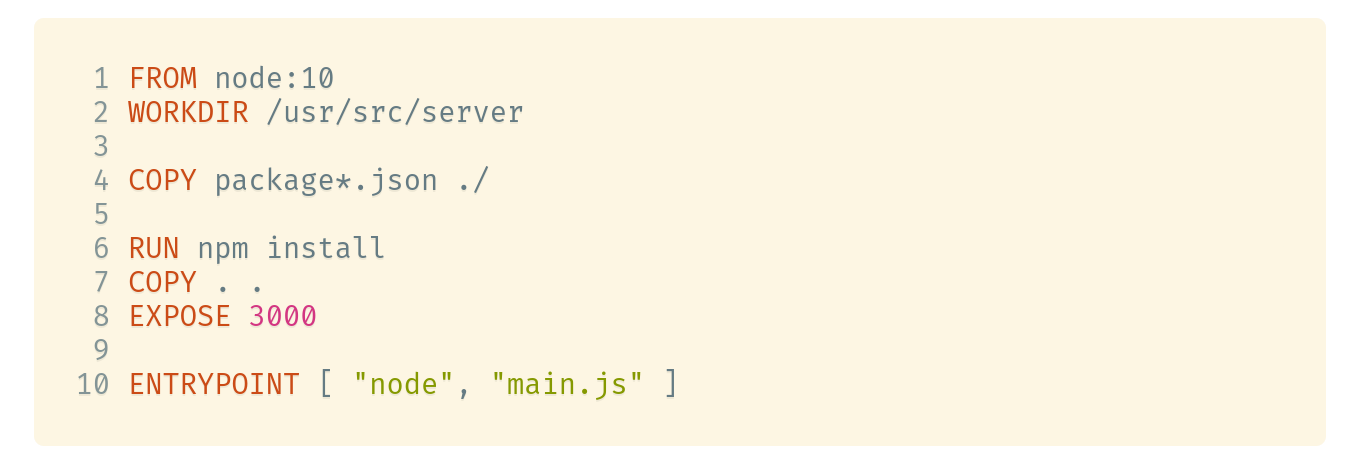
\includegraphics[width=1\textwidth]{images/Docker/dockerfile.png}
        \vspace{-25pt}
        \caption{Beispielhaftes Dockerfile für eine Node.js Web-App}
    \end{center}
\end{code}

\subsection{Container}

Ein Docker-Container führt immer ein zuvor generiertes Docker-Image aus. Dieses Image kann entweder selbstgeneriert sein oder von einer \textbf{Docker-Registry} wie \textit{Docker Hub} kommen, welches Software verschiedenster Herausgeber als fix fertiges Image zur Verfügung stellt.

\subsection{Volume}

Im Allgemeinen ist es Containern nicht möglich, auf das Dateisystem des Hostsystems zuzugreifen. Manchmal ist dies allerdings notwendig, beispielsweise wenn zur Anwendung hochgeladene Bilder gespeichert werden müssen. Damit diese Daten bei einem Neustart des Containers nicht verloren gehen, können \textbf{Volumes} konfiguriert werden, welche es einem Container erlauben, in einem fix festgelegten Ordner auf dem Hostsystem zu lesen und zu schreiben.